\section{Extraction of correlation functions and analysis}\label{sec:corr}
To extract the correlation functions, we first obtain the same-event yields as a function of $\Delta \phi$ and $\Delta y$, defined as 
\begin{equation}
    S(\Delta\phi,\Delta y) = \frac{1}{N_{\rm trig}}\frac{dN^{\rm same}}{d\Delta \phi d\Delta y}
\end{equation}
where $N_{\rm trig}$ is the number of trigger hadrons in the event sample\footnote{This includes those without an associated hadron.  Therefore the integral of $S(\Delta\phi,\Delta y)$ is not necessarily 1, but rather the ratio of the number of associated hadrons in events with a trigger hadron in the event sample to the number of trigger hadrons.}.
Then we obtain the normalized mixed yield, defined as
\begin{equation}
    M(\Delta\phi,\Delta y) = \frac{1}{N^{\rm mix}_{\rm tot}}\frac{dN^{\rm mix}}{d\Delta \phi d\Delta y}(\Delta \phi,\Delta y)
\end{equation}
The correlation function, which is expected to be free of detector effects, is defined as 
\begin{equation}
    C(\Delta\phi,\Delta y) = \frac{S(\Delta\phi,\Delta y)}{M(\Delta\phi,\Delta y)}.
\end{equation}

For the 1D projection $C(\Delta\phi)$ for large rapidity separation, we take the ratios of the the integrals of both the same- and mixed-event yields:
\begin{equation}
    C(\Delta\phi) = \frac{\int_{\Delta y_{\rm min}}^{\Delta y_{\rm max}} d\Delta y  [S(\Delta\phi,\Delta y)]}{\int_{\Delta y_{\rm min}}^{\Delta y_{\rm max}} d\Delta y [M(\Delta\phi,\Delta y)]},
\end{equation}
where we choose $\Delta y_{\rm min}$ and $\Delta y_{\rm min}$ to be 1.5 and 2.5 respectively for this analysis.  
\subsection{Fourier analysis}
\label{sec:fourier}
Fourier transforms are performed on the correlation function $C(\Delta\phi)$.  In principle the coefficients $V_n$ may be compared to predictions made using structure functions.  

\begin{equation}
    f(\Delta\phi) = A(1+2\sum\limits_n V_n\cos (n\Delta\phi))
\end{equation}

\subsection{Ridge yield}
Some theoretical models predict the existence of a bump in the correlation function at $\Delta\phi=0$ [insert reference].  These have been observed in large multiplicity events at CMS in PbPb, $p$Pb, and $pp$  scattering reactions \cite{Khachatryan:2010gv,CMS:2012qk,Khachatryan:2015lva}.  In addition, limits have been set in ALEPH \cite{Lee:2019tmr} and preliminary results from HERA [insert citation] 

Following [insert citation], we use the zero-yield at minimum (ZYAM) procedure to determine the ridge yield, as illustrated in Fig.~\ref{fig:ridge_yield_procedure}.   The first step is fitting the correlation function to a 3rd order Fourier series $f(\Delta\phi)$ (see Sec.~\ref{sec:fourier}.  If the fit function is concave-up at $\Delta\phi=0$, then the yield is zero.  Otherwise, if $f''(0)$ is negative, then the minimum of the function is found, where $f'(\Delta\phi_{\rm min})=0$.  The value of the fit at the minimum is then subtracted from the total correlation function, and then the integral of the correlation function is between $-\Delta\phi_{\rm min}$ and $\Delta\phi_{\rm min}$ is found.  This is then normalized by dividing it by the integral of the correlation function (pre-subtraction) over the full $-\pi$ to $\pi$ range. 

In order to determine upper limits on the ridge yield, we perform a bootstrap procedure \cite{10.1214/aos/1176344552}, in which the values in each bin are randomly modified by a gaussian whose mean is equal to the measured value in the bin, and the sigma is the statistical uncertainty in that bin.  The ridge-yield analysis procedure is repeated on each bootstrap iteration XXXX times, and the upper limits are obtained as the 95th percentile of the yields for the bootstraps.  

\begin{figure}
    \centering
    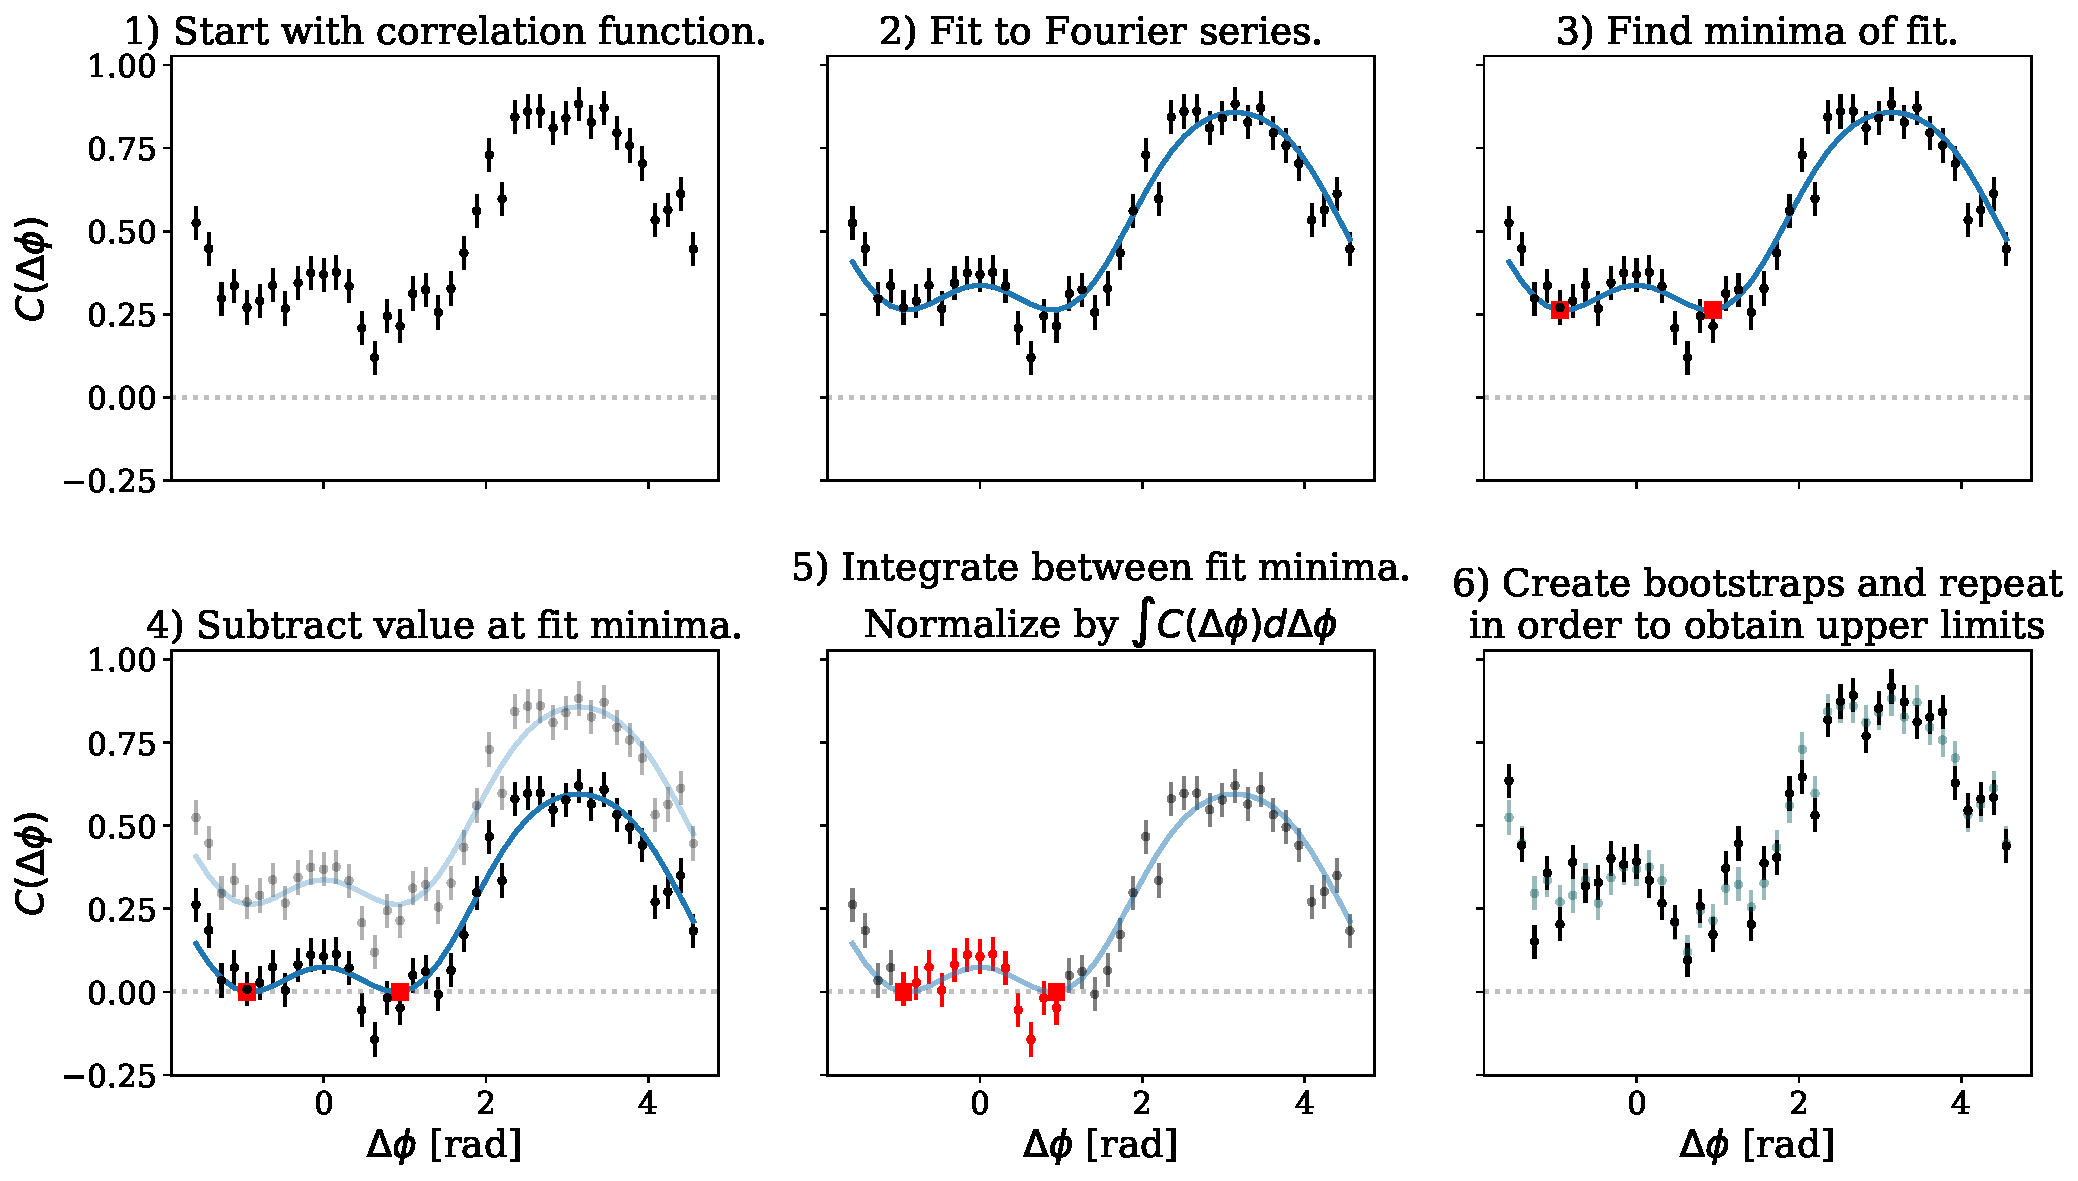
\includegraphics[width=\textwidth]{ridge_yield_procedure.pdf}
    \caption{Illustration of ridge yield procedure}
    \label{fig:ridge_yield_procedure}
\end{figure}


%We took the Fourier transform of the correlation function $C(\Delta\phi)$.  Of particular interest is the parameter $v_2$, defined as the ratio of the $\cos 2\Delta\phi$ coefficient in the Fourier series of the correlation function to that of the constant term.